\documentclass[a4paper, 12pt]{article}

\usepackage[portuges]{babel}
\usepackage[utf8]{inputenc}
\usepackage[margin=1.2in]{geometry}
\usepackage{amsmath}
\usepackage{graphicx}
\usepackage{datetime}
\usepackage{enumerate}
\renewcommand{\baselinestretch}{1.5}

\emergencystretch 1pt%
\setlength{\parindent}{0pt}

\title{EFC1 - Regressão Linear}
\author{Rafael Gonçalves - RA: 186062}

\begin{document}


\maketitle

\section*{Parte I - Atividades teóricas}

\subsection*{Exercício 1}

\begin{enumerate}[a)]
\item
$P(A^C) = 1 - P(A) = 1 - \frac{1}{3} = \frac{2}{3}$

\item
$P(A^C \cup B) = P(A^C) + P(B) - P(A^CB) = P(A^C) + P(B) - (P(B) - P(AB)) = P(A^C) + P(AB) = \frac{2}{3} + \frac{1}{6} = \frac{5}{6}$

\item
$P(A \cup B^C) = P(A) + P(B^C) - P(AB^C) = P(B^C) + P(AB) = (1 - P(B)) + P(AB) = (1 - \frac{1}{4}) + \frac{1}{6} = \frac{11}{12}$

\item
    $P(AB^C) = P(A) + P(B^C) - P(A \cup B^C) = \frac{1}{3} + \frac{3}{4} - \frac{11}{12} = \frac{2}{12} = \frac{1}{6}$

\item
    $P(A^C \cup B^C) = 1 - P(AB) = 1 - \frac{1}{6} = \frac{5}{6}$

\end{enumerate}

\subsection*{Exercício 2}

\begin{enumerate}[a)]
\item
$$
    F_X(x) = P(X \leq x) = \int\limits_{-\infty}^x f_X(\xi) d\xi = \int\limits_{-\infty}^x \frac{1}{2} d\xi = \left[ \frac{1}{2}\xi \right]^x_0 = \frac{1}{2} x, \forall X \in [0, 2]
$$

\item
$E\{X\} = \int\limits_{-\infty}^{\infty} xf_X(x)dx = \int\limits_0^2 \frac{1}{2}x dx = \left[\frac{x^2}{4}\right]^2_0 = 1$

$E\{X^2\} = \int\limits_{-\infty}^{\infty} x^2f_X(x)dx = \int\limits_0^2 \frac{1}{2}x^2 dx = \left[\frac{x^3}{6}\right]^2_0 = \frac{4}{3}$

$E\{X^3\} = \int\limits_{-\infty}^{\infty} x^3f_X(x)dx = \int\limits_0^2 \frac{1}{2}x^3 dx = \left[\frac{x^4}{8}\right]^2_0 = 2$
\end{enumerate}

\subsection*{Exercício 3}

\begin{enumerate}[a)]
\item
$X_2$, pois quanto mais próximo da distribuição uniforme, mais difícil é acertar o resultado de um evento aleatório "chutando um valor", ou seja, a variável aleatória $X_2$ carrega mais informação que a variável aleatória $X_1$, pois neste último eu poderia supor que o resultado será sempre 3 com uma taxa de acertos de 40\% contra uma taxa de acertos de 25\% para qualquer valor estimado para $X_2$ se não tivermos nenhuma informação \em a priori\em .


\item
$H(X_1) = - \sum\limits_x p(X_1)log_2[p(X_1)] = -[0,1(-3,32) + 0,2(-2,32) + 0,3(-1,74) + 0,4(-1,32)] = 1,85$

$H(X_2) = - \sum\limits_x p(X_2)log_2[p(X_2)] = - [0,25 (-2) + 0,25 (-2) + 0,25 (-2) + 0,25(-2)] = 2$


\item
$D(P_1 || P_2) = \sum\limits_x p(X_1)log_2\left[\frac{p(X_1)}{p(X_2)}\right] = 0,1(-1,32) + 0,2(-0,32) + 0,3(0,26) + 0,4(0,68) = 0,15$

$D(P_2 || P_1) = \sum\limits_x p(X_2)log_2\left[\frac{p(X_2)}{p(X_1)}\right] = 0,25(1.32 +  0.32 - 0.26 -0.68) = 0,18$

\end{enumerate}

\subsection*{Exercício 4}

\begin{enumerate}[a)]
\item
    $\mathcal{L}(\mu) = p(x|\mu) = \frac{p(x\mu)}{p(\mu)} = p(x) = f_\mu(x)$

\item
    $\mathcal{L}(\mu) = p(\mathbf{x}|\mu) = \prod \limits _{k=1} ^{N} p(x_k|\mu) = \prod\limits_{k=1}^{N} \frac{p(x_k|\mu)}{p(\mu)} = \prod\limits_{k=1}^{N} f_\mu(x_k)$

\item

    $\mu_{ML} = arg max_\mu \mathcal{L}(\mu) = arg max_\mu ln \left [ \prod\limits_{k=1}^{N} f_\mu(x_k) \right ] =arg max_\mu \sum \limits_{k=1}^{N} ln [ f_\mu (x_k) ] = arg max_\mu \sum \limits_{k=1}^{N} ln \left [ \frac{1}{\sigma \sqrt{2\pi }} e^{- \frac{1}{2} \left (\frac{x - \mu}{\sigma} \right ) ^2} \right ] =  arg max_\mu \sum \limits_{k=1}^{N} \left [ ln \left ( \frac{1}{\sigma \sqrt{2\pi }} \right ) - \frac{1}{2} \left (\frac{x - \mu}{\sigma} \right )^2 \right ] =$
        
        $arg max_\mu \sum \limits_{k=1}^{N} - \frac{1}{2} \left (\frac{x - \mu}{\sigma} \right )^2 - N ln ( \sigma \sqrt{2 \pi} ) = argmax _\mu A \iff \frac{dA}{d\mu} = 0 \Rightarrow$

        $\sum \limits _{k=1} ^N \frac{-2}{2} \left ( \frac{x - \mu}{\sigma} \right ) ( -1 ) = 0 \Rightarrow \sum \limits _{k=1}^N x_k - N\mu = 0 \Rightarrow$
        $\mu_{ML} = \frac{1}{N} \sum \limits _{k=1}^{N} x_k $

\end{enumerate}

\newpage

\section*{Parte II - Atividade computacional}

\subsection*{a) Solução fechada com MMQ}

$
\mathbf{X} =\begin{bmatrix}
    \mathbf{x_1} \\
    \mathbf{x_2} \\
    \vdots \\
    \mathbf{x_N}
\end{bmatrix}
$
\hspace{2em}
$
\boldsymbol{\Phi} = \boldsymbol{\Phi}(\mathbf{X}) = \begin{bmatrix}
    1 & \mathbf{x_1} \\
    1 & \mathbf{x_2} \\
    &\vdots \\
    1 & \mathbf{x_N}
\end{bmatrix}
$
\hspace{2em}
$
\mathbf{y} =\begin{bmatrix}
    y_1 \\
    y_2 \\
    \vdots \\
    y_N
\end{bmatrix}
$

\vspace{1em}

Modelo:
\begin{equation}
    \mathbf{\hat{y}} = \mathbf{\hat{y}}(\mathbf{X}) = \boldsymbol{\Phi}\mathbf{w}
\end{equation}

Solução ótima com o método de mínimos múltiplos quadrados (MMQ):
\begin{equation}
    \mathbf{w} = (\boldsymbol{\Phi}^T\boldsymbol{\Phi})^{-1}\boldsymbol{\Phi}^T\mathbf{y}
\end{equation}

Raiz quadrada do erro quadrático médio (RMSE) para o modelo treinado com o conjunto de treino:

$ RMSE _{train} = 15.3702$
\hspace{2em}
$ RMSE _{test} = 14.2495$

Resultado no conjunto de teste:

\begin{figure}[h!]
    \centering
    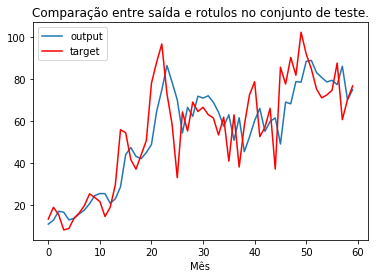
\includegraphics[width=9cm]{images/raw.png}
    \caption{Saída prevista pelo modelo (azul) em comparação com valores reais dos últimos 5 anos (60 meses).}
\end{figure}

\subsection*{b) Seleção de atributos usando wrapper (backward elimination), validação cruzada (k-fold) e regularização L2}

Solução por MMQ com regularização ridge (L2):
\begin{equation}
    \mathbf{w} = (\boldsymbol{\Phi}^T\boldsymbol{\Phi} + \lambda\mathbf{I'})^{-1}\boldsymbol{\Phi}^T\mathbf{y}
\end{equation}

\begin{figure}[h!]
    \centering
    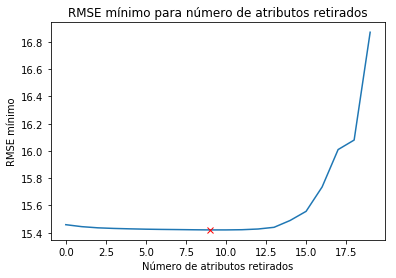
\includegraphics[width=8cm]{images/backward.png}
    \caption{Menor RMSE para cada passo do wrapper (atributo retirado).}
\end{figure}

Modelo escolhido pelo wrapper utilizando k-fold com 5 pastas:

N de atributos removidos: $9 \quad \lambda: 10000 \quad RMSE_{CV}: 15.4201 \quad RMSE_{test}: 14.4200$

Atributos escolhidos: 0 (bias) , 1, 2, 3, 4, 5, 6, 8, 9, 11, 18, 20

\begin{figure}[h!]
    \centering
    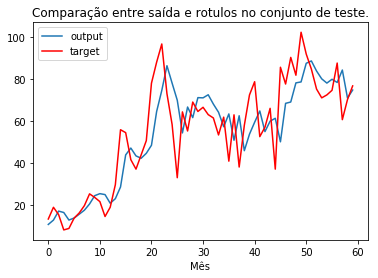
\includegraphics[width=9cm]{images/wrapper.png}
    \caption{Saída prevista pelo modelo (azul) em comparação com valores reais dos últimos 5 anos (60 meses) com seleção de atributos usando wrapper.}
\end{figure}

\begin{table}[]
    \centering
    \caption{RMSE mínimo e respectivo lambda para cada número de atributos retirados.}
\begin{tabular}{lll}
N atributos retirados & min RMSE & lambda \\
0                     & 15.4585 & 30000 \\
1                     & 15.4441 & 30000 \\
2                     & 15.4355 & 30000 \\
3                     & 15.4311 & 30000 \\
4                     & 15.4280 & 30000 \\
5                     & 15.4255 & 30000 \\
6                     & 15.4238 & 10000 \\
7                     & 15.4226 & 10000 \\
8                     & 15.4212 & 10000 \\
9                     & 15.4201 & 10000 \\
10                    & 15.4202 & 10000 \\
11                    & 15.4216 & 10000 \\
12                    & 15.4268 & 10000 \\
13                    & 15.4392 & 6000  \\
14                    & 15.4893 & 6000  \\
15                    & 15.5565 & 1000  \\
16                    & 15.7354 & 0     \\
17                    & 16.0103 & 0     \\
18                    & 16.0801 & 0     \\
19                    & 16.8718 & 0
\end{tabular}
\end{table}


\subsection*{c) Seleção de atributos usando filtro (correlação de Pearson)}

\begin{figure}[h!]
    \centering
    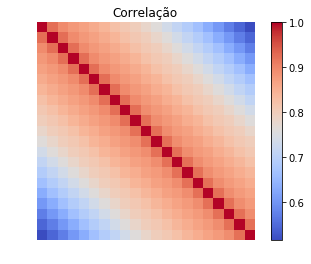
\includegraphics[width=7cm]{images/corr.png}
    \caption{Matriz de correlação, onde uma cor mais avermelhada significa uma correlação maior (dados foram alinhados na matriz de forma que a primeira linha e coluna correspondem ao rótulo e as próximas linhas e colunas correspondem aos atributos - mês anterior até 20 meses atrás).}
\end{figure}

Modelo escolhido pelo filtro (11 atributos com maior correlação):

Atributos selecionados: 0 (bias) , 1, 2, 3, 4, 5, 6, 7, 8, 9, 10, 11

$\lambda: 10000 \quad\quad RMSE_{CV}: 15.7380 \quad\quad RMSE_{test}: 13.8367$

\begin{figure}[h!]
    \centering
  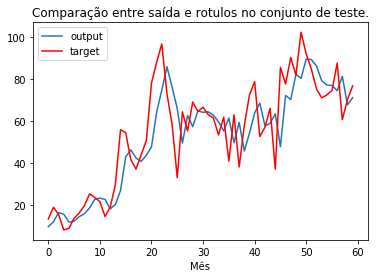
\includegraphics[width=9cm]{images/filter.png}
    \caption{Saída prevista pelo modelo (azul) em comparação com valores reais dos últimos 5 anos (60 meses) com seleção de atributos usando filtro.}
\end{figure}

\begin{figure}[h!]
    \centering
  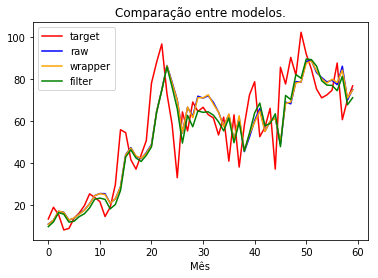
\includegraphics[width=9cm]{images/comparison.png}
    \caption{Saída prevista por cada modelo: azul - modelo inicial com 20 atributos, RMSE = 14.2495; amarelo - modelo criado usando wrapper, RMSE = 14.1138; verde - modelo criado usando filtro, RMSE = 13.8367;  em comparação com valores reais (vermelho) dos últimos 5 anos (60 meses).}
\end{figure}


\hspace{2em} Ambas as estratégias de seleção de atributos em conjunto com a regularização L2 mostraram melhoria em relação ao uso de todos os 20 atributos sem regularização. Podemos observar que embora o erro de validação tenha sido menor na abordagem com seleção de atributos usando wrapper, o erro no conjunto de testes foi menor na abordagem de filtro. Isso pode ser consequência de o modelo utilizado ser linear e portanto se beneficiar diretamente por atributos que tenha uma correlação com os rótulos.

\hspace{2em} Também vale notar que o modelo gerado com seleção de atributos pelo wrapper leva em consideração o erro da validação para escolher quais atributos usar, enquanto que o modelo gerado pelo filtro não leva em conta o erro da validação para seleção de atributos, apenas a correlação entre cada atributo e o rótulo e, sendo assim, faz sentido que o modelo do wrapper apresente um erro menor de validação em comparação ao modelo gerado usando filtro. Em todo o caso o resultado nos mostra que o modelo que obteve um melhor desempenho em dados novos foi o modelo gerado com o filtro e é o modelo que deve ser usado em uma aplicação - provavelmente terá melhor desempenho.

\end{document}
